\documentclass{article}
\usepackage{subfiles}
\usepackage{graphicx}
\usepackage{hyperref}
\usepackage{amsfonts}
\usepackage{amsmath}
\usepackage{amssymb}
\usepackage{amsthm}
\usepackage{enumitem}
\usepackage{caption}
\usepackage{tikz}
\usepackage{graphicx}
\usepackage{float}
\usepackage{url}
\hypersetup{
    colorlinks=true,
    linktoc=all,
    linkcolor=blue,
}


\begin{document}

\newpage
    \subfile{Sources/titlepage}
\newpage

\newpage
    \tableofcontents
\newpage

\section{Neural Networks}
\subsection{Graph Neural Networks}

\section{Graph Data Structure}
A \emph{graph} $G$ [\autoref{fig:example-graph}] is a non-linear data structure consisting of vertices and edges. The vertices are sometimes also referred to as nodes and the edges are arcs that connect any two nodes in the graph. Graphs are used to represent relationships between different entities and have applications in many fields including Computer Science, Physics, Biology, Chemistry, Optimization Theory and many more.

\begin{figure}[H]
    \centering
    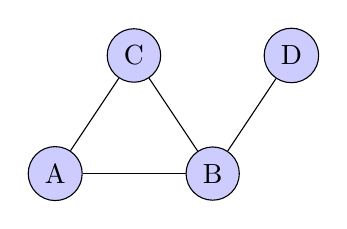
\begin{tikzpicture}
        % Define the vertices
        \node[circle, draw, fill=blue!20] (A) at (0,0) {A};
        \node[circle, draw, fill=blue!20] (B) at (2,0) {B};
        \node[circle, draw, fill=blue!20] (C) at (1,1.5) {C};
        \node[circle, draw, fill=blue!20] (D) at (3,1.5) {D};
        
        % Define the edges
        \draw (A) -- (B);
        \draw (A) -- (C);
        \draw (B) -- (C);
        \draw (B) -- (D);
    \end{tikzpicture}
    \caption{A simple graph}
    \label{fig:example-graph}
\end{figure}

\subsection{Formal Definition}
A graph is formally defined as a tuple $G = (V, E)$, where:
\begin{itemize}
    \item $V$ is a finite set of vertices (or nodes).
    \item $E$ is a set of edges, where each edge is an unordered pair of distinct vertices from $V$. Thus, $E \subseteq \{\{u, v\} \mid u, v \in V \text{ and } u \neq v\}$.
\end{itemize}

\subsection{Types of Graphs}
Graphs can be classified into various types based on their properties, including:
\begin{itemize}
    \item \textbf{Directed Graph} [\autoref{fig:directed-graph}]: A graph in which the edges have a direction, i.e., each edge is an ordered pair of vertices.
    
    \begin{figure}[H]
    \centering
    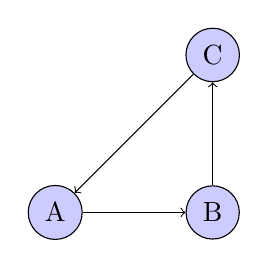
\begin{tikzpicture}
        % Vertices
        \node[circle, draw, fill=blue!20] (A) at (0,0) {A};
        \node[circle, draw, fill=blue!20] (B) at (2,0) {B};
        \node[circle, draw, fill=blue!20] (C) at (2,2) {C};
        
        % Directed edges
        \draw[->] (A) -- (B);
        \draw[->] (B) -- (C);
        \draw[->] (C) -- (A);
    \end{tikzpicture}
    \caption{Directed graph example.}
    \label{fig:directed-graph}
    \end{figure}

    \item \textbf{Undirected Graph} [\autoref{fig:undirected-graph}]: A graph in which the edges do not have a direction, i.e., each edge is an unordered pair of vertices.
    
    \begin{figure}[H]
    \centering
    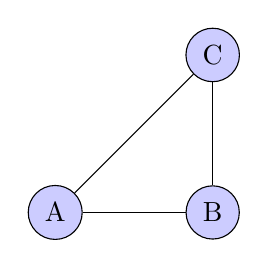
\begin{tikzpicture}
        % Vertices
        \node[circle, draw, fill=blue!20] (A) at (0,0) {A};
        \node[circle, draw, fill=blue!20] (B) at (2,0) {B};
        \node[circle, draw, fill=blue!20] (C) at (2,2) {C};
        
        % Undirected edges
        \draw (A) -- (B);
        \draw (B) -- (C);
        \draw (C) -- (A);
    \end{tikzpicture}
    \caption{Undirected graph example.}
    \label{fig:undirected-graph}
    \end{figure}
    
    \item \textbf{Weighted Graph} [\autoref{fig:weighted-graph}]: A graph in which a weight (or cost) is associated with each edge.
    
    \begin{figure}[H]
    \centering
    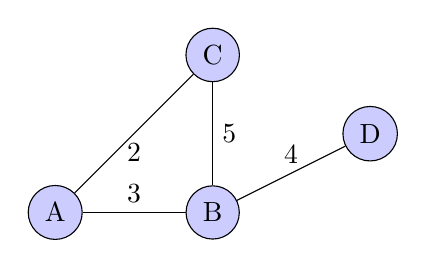
\begin{tikzpicture}
        % Vertices
        \node[circle, draw, fill=blue!20] (A) at (0,0) {A};
        \node[circle, draw, fill=blue!20] (B) at (2,0) {B};
        \node[circle, draw, fill=blue!20] (C) at (2,2) {C};
        \node[circle, draw, fill=blue!20] (D) at (4,1) {D};
        
        % Edges with weights
        \draw (A) -- node[above] {3} (B);
        \draw (B) -- node[right] {5} (C);
        \draw (C) -- node[below] {2} (A);
        \draw (B) -- node[above] {4} (D);
    \end{tikzpicture}
    \caption{Weighted graph example.}
    \label{fig:weighted-graph}
    \end{figure}
    
    \item \textbf{Simple Graph} [\autoref{fig:simple-graph}]: A graph with no loops (edges connecting a vertex to itself) and no multiple edges (more than one edge connecting the same pair of vertices).
    
    \begin{figure}[H]
    \centering
    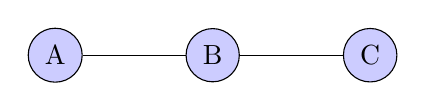
\begin{tikzpicture}
        % Vertices in a straight line
        \node[circle, draw, fill=blue!20] (A) at (0,0) {A};
        \node[circle, draw, fill=blue!20] (B) at (2,0) {B};
        \node[circle, draw, fill=blue!20] (C) at (4,0) {C};
        
        % Edges
        \draw (A) -- (B);
        \draw (B) -- (C);
    \end{tikzpicture}
    \caption{Simple graph example.}
    \label{fig:simple-graph}
    \end{figure}
    
    \item \textbf{Complete Graph} [\autoref{fig:complete-graph}]: A graph in which there is exactly one edge between each pair of distinct vertices.
    
    \begin{figure}[H]
    \centering
    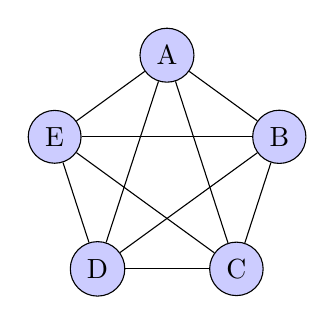
\begin{tikzpicture}
        % Vertices
        \node[circle, draw, fill=blue!20] (A) at (90:1.5cm) {A};
        \node[circle, draw, fill=blue!20] (B) at (18:1.5cm) {B};
        \node[circle, draw, fill=blue!20] (C) at (-54:1.5cm) {C};
        \node[circle, draw, fill=blue!20] (D) at (234:1.5cm) {D};
        \node[circle, draw, fill=blue!20] (E) at (162:1.5cm) {E};
        
        % Complete edges
        \foreach \from/\to in {A/B, A/C, A/D, A/E, B/C, B/D, B/E, C/D, C/E, D/E}
            \draw (\from) -- (\to);
    \end{tikzpicture}
    \caption{Complete graph example.}
    \label{fig:complete-graph}
    \end{figure}

    
    \item \textbf{Bipartite Graph} [\autoref{fig:bipartite-graph}]: A graph whose vertices can be divided into two disjoint sets $U$ and $W$ such that every edge connects a vertex in $U$ to a vertex in $W$.
    
    \begin{figure}[H]
    \centering
    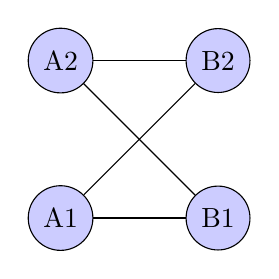
\begin{tikzpicture}
        % Vertices
        \node[circle, draw, fill=blue!20] (A1) at (0,0) {A1};
        \node[circle, draw, fill=blue!20] (A2) at (0,2) {A2};
        \node[circle, draw, fill=blue!20] (B1) at (2,0) {B1};
        \node[circle, draw, fill=blue!20] (B2) at (2,2) {B2};
        
        % Bipartite edges
        \draw (A1) -- (B1);
        \draw (A1) -- (B2);
        \draw (A2) -- (B1);
        \draw (A2) -- (B2);
    \end{tikzpicture}
    \caption{Bipartite graph example.}
    \label{fig:bipartite-graph}
\end{figure}
    
\end{itemize}

\subsection{Graph Representation}
Graphs can be represented in various ways, including:
\begin{itemize}
    \item \textbf{Adjacency Matrix} [\autoref{fig:adjacency-matrix}]: A square matrix $A$ of size $|V| \times |V|$ where $A_{ij} = 1$ if there is an edge between vertices $v_i$ and $v_j$, and $A_{ij} = 0$ otherwise.
    
   \begin{figure}[H]
    \centering
    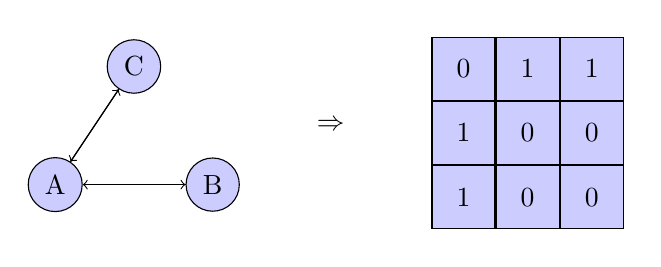
\begin{tikzpicture}
        % Define the vertices
        \node[circle, draw, fill=blue!20] (A) at (0,0) {A};
        \node[circle, draw, fill=blue!20] (B) at (2,0) {B};
        \node[circle, draw, fill=blue!20] (C) at (1,1.5) {C};
        
        % Define the edges
        \draw[->] (A) -- (B);
        \draw[->] (A) -- (C);
        \draw[->] (B) -- (A);
        \draw[->] (C) -- (A);
        
        % Adjacency matrix
        \node (RA) at (3.5,0.75) {$\Rightarrow$};

        \matrix (A) [nodes={draw, minimum size=0.8cm, fill=blue!20}, right=6cm, below=-2cm] {
            \node{0}; & \node{1}; & \node{1}; \\
            \node{1}; & \node{0}; & \node{0}; \\
            \node{1}; & \node{0}; & \node{0}; \\
        };
        
    \end{tikzpicture}
    \caption{Adjacency Matrix representation.}
    \label{fig:adjacency-matrix}
    \end{figure}
    
    \item \textbf{Adjacency List} [\autoref{fig:adjacency-list-undirected}]: An array of lists. The array contains a list for each vertex, and each list contains the vertices that are adjacent to the corresponding vertex.
    
\begin{figure}[H]
    \centering
    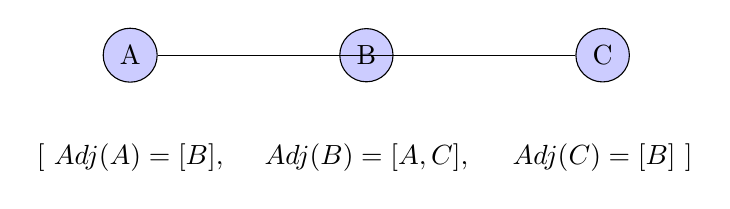
\begin{tikzpicture}
        % Define the vertices
        \node[circle, draw, fill=blue!20] (A) at (0,0) {A};
        \node[align=center, below] at (0, -1) {[ $Adj(A)=[B]$,};
        
        \node[circle, draw, fill=blue!20] (B) at (3,0) {B};
        \node[align=center, below] at (3, -1) {$Adj(B)=[A,C]$,};
        
        \node[circle, draw, fill=blue!20] (C) at (6,0) {C};
        \node[align=center, below] at (6, -1) {$Adj(C)=[B]$ ]};
        
        % Define the edges (undirected)
        \draw (A) -- (B);
        \draw (A) -- (C);
        \draw (B) -- (C);
        
    \end{tikzpicture}
    \caption{Adjacency List representation for an undirected graph.}
    \label{fig:adjacency-list-undirected}
\end{figure}
    
\end{itemize}


\section{Graph Similarity Problem}

The \emph{graph similarity problem} involves determining the degree of similarity between two graphs. This problem has numerous applications in pattern recognition, computer vision, bioinformatics, and other fields. One common method to quantify graph similarity is through the \emph{graph edit distance} (GED).

\subsection{Graph Edit Distance (GED)}

The \emph{graph edit distance} between two graphs $G_1 = (V_1, E_1)$ and $G_2 = (V_2, E_2)$ is defined as the minimum cost required to transform $G_1$ into $G_2$ using a sequence of atomic operations. Formally, let $\Sigma$ be the set of all possible edit operations, and let $c: \Sigma \to \mathbb{R}^+$ be a cost function that assigns a positive real number to each operation. The GED is then given by:

\[
\text{GED}(G_1, G_2) = \min_{\sigma \in \Sigma^*} \sum_{o \in \sigma} c(o)
\]

where $\Sigma^*$ denotes the set of all finite sequences of operations from $\Sigma$, and $o$ represents an individual operation within a sequence $\sigma$.

The computation of GED is known to be \textbf{NP-HARD} \cite{NP_HARDNESS}, indicating that finding the exact minimum edit distance between two graphs is computationally intensive.

\subsection{Atomic Operations}

The basic atomic operations typically includes:

\begin{itemize}
    \item \textbf{Vertex Insertion}: Inserting a new vertex $v$ into the graph.
    \item \textbf{Vertex Deletion}: Deleting an existing vertex $v$ from the graph.
    \item \textbf{Edge Insertion}: Inserting a new edge $e = \{u, v\}$ into the graph.
    \item \textbf{Edge Deletion}: Deleting an existing edge $e = \{u, v\}$ from the graph.
\end{itemize}

To demonstrate the Graph Edit Distance (GED), consider pair of graphs represented in \ref{fig:ged-graphs}:

\begin{figure}[H]
    \centering
    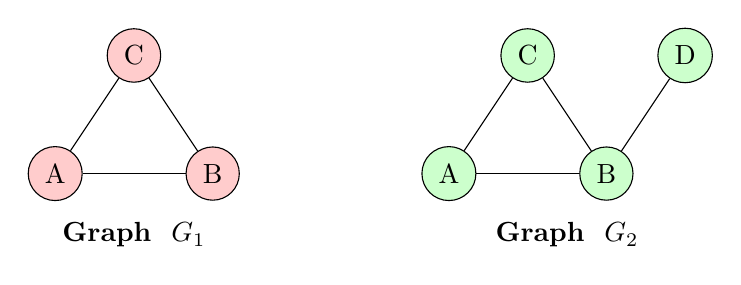
\begin{tikzpicture}
        % Define the vertices for G1
        \node[circle, draw, fill=red!20] (A1) at (0,0) {A};
        \node[circle, draw, fill=red!20] (B1) at (2,0) {B};
        \node[circle, draw, fill=red!20] (C1) at (1,1.5) {C};
        
        % Define the edges for G1
        \draw (A1) -- (B1);
        \draw (A1) -- (C1);
        \draw (B1) -- (C1);
        
        % Annotations for G1
        \node[align=center, below] at (1, -0.5) {\textbf{Graph } $G_1$};
        
        % Define the vertices for G2
        \node[circle, draw, fill=green!20] (A2) at (5,0) {A};
        \node[circle, draw, fill=green!20] (B2) at (7,0) {B};
        \node[circle, draw, fill=green!20] (C2) at (6,1.5) {C};
        \node[circle, draw, fill=green!20] (D2) at (8,1.5) {D};
        
        % Define the edges for G2
        \draw (A2) -- (B2);
        \draw (A2) -- (C2);
        \draw (B2) -- (C2);
        \draw (B2) -- (D2);
        
        % Annotations for G2
        \node[align=center, below] at (6.5, -0.5) {\textbf{Graph } $G_2$};
        
        
    \end{tikzpicture}
    \caption{Pair of graphs to demonstre Graph Edit Distance.}
    \label{fig:ged-graphs}
\end{figure}

In this example, graph $G_1$ has vertex set $V_1 = \{A, B, C\}$ and edge set $E_1 = \{\{A, B\}, \{A, C\}, \{B, C\}\}$, while graph $G_2$ has vertex set $V_2 = \{A, B, C, D\}$ and edge set $E_2 = \{\{A, B\}, \{A, C\}, \{B, C\}, \{B, D\}\}$. The transformation (which cost is lowest) from $G_1$ to $G_2$ involves: Inserting the vertex $D$ and Inserting the edge $\{B, D\}$. If we assign a cost of 1 to each operation the total cost (GED) is: $1+1=2$.

\section{SimGNN}
\section{Bottleneck Loading GPU Problem}
\section{Dataset Generation}
\section{State of the Art Review}


\bibliographystyle{plain}
\bibliography{References}


\end{document}
